\begin{center}
    \begin{tcolorbox}[width=3.5in]
        Find the {\bfseries\itshape domain} of a continuous function by
        drawing the ``shadow'' of the graph onto the $x$-axis.
    \end{tcolorbox}
\end{center}

\begin{center}
    \begin{tcolorbox}[width=3.5in]
        Find the {\bfseries\itshape range} of a continuous function by
        drawing the ``shadow'' of the graph onto the $y$-axis.
    \end{tcolorbox}
\end{center}


\begin{myExample}{
    Find the domain and range of this relation.
    \begin{center}
        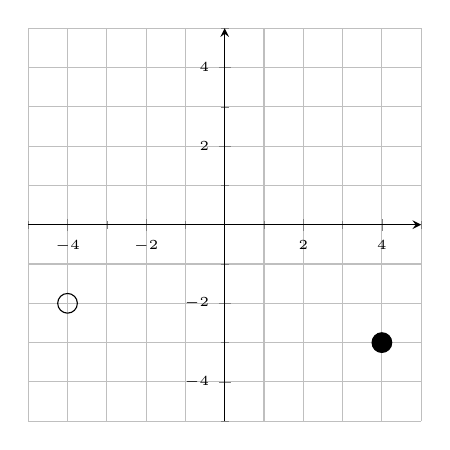
\begin{tikzpicture}
            \begin{axis}[
                width=3in,
                grid=both,
                axis x line = middle,axis y line = middle,
                axis equal image,
                xtick distance = 2, ytick distance = 2, 
                minor tick num = 1,
                xmin = -5, xmax=5,
                ymin = -5, ymax=5,
                tick label style = {font=\tiny},
                ]
                \addplot[mark=o,mark size=0.125cm,] coordinates { (-4,-2) };
                \addplot[mark=*,mark size=0.125cm,] coordinates { (4,-3) };
            \end{axis}
        \end{tikzpicture}
    \end{center}
}
    \vspace{6in}
\end{myExample}

\begin{taggedblock}{on-level}
\begin{myExample}{
    Find the domain and range of this relation.
    \begin{center}
        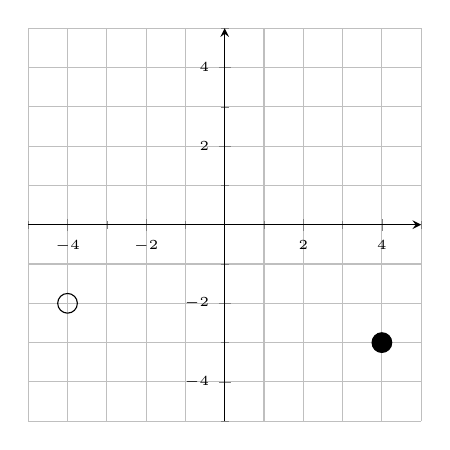
\begin{tikzpicture}
            \begin{axis}[
                width=3in,
                grid=both,
                axis x line = middle,axis y line = middle,
                axis equal image,
                xtick distance = 2, ytick distance = 2, 
                minor tick num = 1,
                xmin = -5, xmax=5,
                ymin = -5, ymax=5,
                tick label style = {font=\tiny},
                ]
                \addplot[mark=o,mark size=0.125cm,] coordinates { (-4,-2) };
                \addplot[mark=*,mark size=0.125cm,] coordinates { (4,-3) };
            \end{axis}
        \end{tikzpicture}
    \end{center}
}
    \vspace{6in}
\end{myExample}
\end{taggedblock}

\begin{taggedblock}{pre-AP}
\begin{myExample}{
    Find the domain and range of this relation.
    \begin{center}
        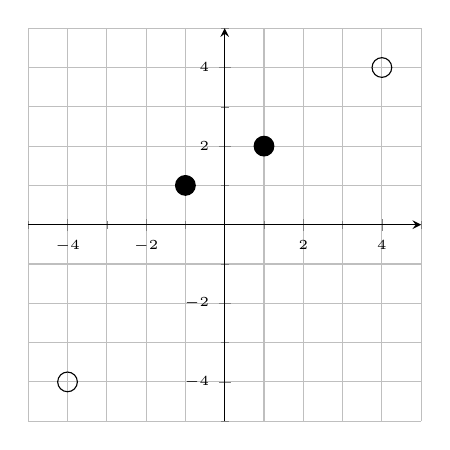
\begin{tikzpicture}
            \begin{axis}[
                width=3in,
                grid=both,
                axis x line = middle,axis y line = middle,
                axis equal image,
                xtick distance = 2, ytick distance = 2, 
                minor tick num = 1,
                xmin = -5, xmax=5,
                ymin = -5, ymax=5,
                tick label style = {font=\tiny},
                ]
                \addplot[mark=o,mark size=0.125cm,] coordinates { (-4,-4) };
                \addplot[mark=*,mark size=0.125cm,] coordinates { (-1,1) };
                \addplot[mark=*,mark size=0.125cm,] coordinates { (1,2) };
                \addplot[mark=o,mark size=0.125cm,] coordinates { (4,4) };
            \end{axis}
        \end{tikzpicture}
    \end{center}
}
    \vspace{5.5in}
\end{myExample}
\end{taggedblock}
